\section{Memoria di massa}\label{mass memory}
In questo capitolo iniziamo ad occuparci della gestione della memoria secondaria. Discuteremo innanzitutto il tipo di periferiche con il quale andremo a lavorare per poi passare ad alcuni algoritmi per lo scheduling e l'utilizzo ottimale di tali periferiche. Passeremo poi ad approfondire alcuni aspetti sulla gestione di questi dispositivi e del loro spazio di archiviazione (in particolare dello \textit{swapping}, discusso già nel paragrafo \ref{swapping}). Infine discuteremo su alcuni metodi per l'immagazzinamento di molti dati, come le strutture RAID.

\subsection{Tipi di memoria secondaria}
Iniziamo con il distinguere due tipi di supporti di dati più comuni: stiamo parlando dei dischi rigidi, chiamati anche HDD, e delle schede basate su una tecnologia moderna chiamate NVM

\subsubsection{HDD}\label{seek}
L'HDD, che sta per \textit{Hard Disk Device}, è quello che comunemente viene chiamato \textbf{disco rigido}. Questa unità è composta da diversi dischi magnetici, una sopra l'altro. Facendo riferimento all'immagine \ref{fig:HDD}, possiamo notare che ogni disco è formato da delle \textbf{tracce}, ovvero il cerchio a distanza $\overline{R}$ dal centro. Ogni traccia è composta da diversi \textbf{settori}. L'insieme delle tracce a distanza $\overline{R}$ dal centro del disco è detto \textbf{cilindro}.
\begin{figure}[h]
    \centering
    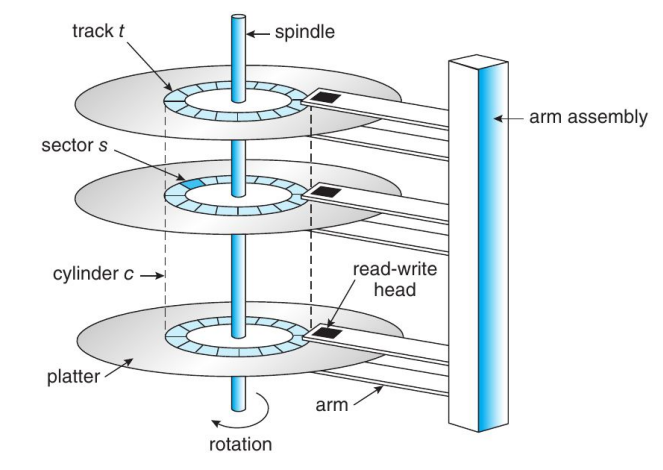
\includegraphics[width = .6\textwidth]{../res/imgs/mass memory/HDD.png}
    \caption{Schema ad alto livello di un disco rigido.}
    \label{fig:HDD}
\end{figure}
Al fine di riuscire a leggere le informazioni dei dischi, questi girano e una "testina" (\textit{arm}, ce n'è una per ogni disco) si appoggia sulla traccia e legge l'informazione.

Essendo uno spostamento fisico, la lettura dal disco è abbastanza lenta in quanto è necessario che la testina raggiunga la traccia del disco necessaria, a questo punto il disco gira fino a che non si è raggiunta l'informazione cercata. Il tempo di posizionamento sulla traccia (o settore) è detto \textbf{seek time} mentre il tempo dovuto alla rotazione del disco è detto \textbf{rotational latency}. Possiamo quindi cercare di calcolare la performance di un HDD attraverso delle medie aritmetiche:
\vspace{-5px}
\begin{itemize}
\setlength{\itemsep}{-.15 em}
    \item \textit{average access time}: il tempo medio di accesso si calcola sommando l'\textit{average seek time} e l'\textit{average latency};
    \item \textit{average I/O time} si calcola sommando il valore trovato nel punto precedente a al tempo di trasferimento e all'\textit{overhead} di un potenziale controllore elettrico/periferica: $AVG\_Access\_Time + \frac{Amount\_to\_Transfer}{Transfer\_rate} + Controller\_Overhead$.
\end{itemize}

% 
\subsubsection*{Esercizio}
Prendiamo in considerazione la situazione di dover trasferire un blocco da 4KB su un disco che gira a 7200 RPM (\textit{rotation per minute}) con un \textit{average seek time} di 5 millisecondi e un \textit{transfer rate} di 1Gigabit/sec con un \textit{overhead} del controllore di 0.1 millisecondi. Seguendo la formula del secondo punto, dobbiamo trovare \textit{average Access Time} e \textit{Transfer Time} dato che il \textit{Controller Overhead} già lo conosciamo.
\begin{itemize}
\setlength{\itemsep}{-.15 em}
    \item \textit{Average Access Time} = \textit{average Seek Time} (=5ms) + \textit{Average Latency}. Per calcolare quest'ultima si fa:$\frac{1}{2}\cdot\frac{60}{7200}\cdot10^3 = 10^3 \cdot \frac{30}{7200}$. Di conseguenza l'\textit{Average Access Time} diventa: $5 + 4.17$ms = 9.17ms.
    \item \textit{Transfer Time} = $\frac{\text{\textit{Amount to Transfer}}}{\text{\textit{Transfer rate}}}$ = $\frac{4KB}{1 Gb/sec} = \frac{4KB}{\frac{1}{8}GB/sec} = \frac{32KB}{1024^2 KB/sec} = 0.031$ms
\end{itemize}
A questo punto sommiamo i due risultati all'\textit{overhead} e otteniamo $9.301$ms.

% 
\subsubsection{NVM}\label{NVM}
\begin{wrapfigure}{o}{.30\textwidth}
  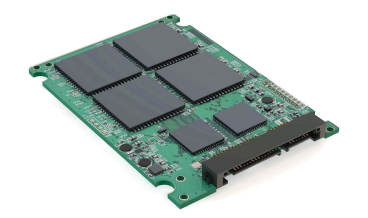
\includegraphics[width = \linewidth]{../res/imgs/mass memory/NVM.png}
  \label{fig:NVM}
\end{wrapfigure}
I dispositivi NVM (\textit{NonVolatile Memory}, ovvero memoria non volatile) sono anche chiamati \textbf{SSD}, che sta per \textit{Solid-State Disk}. Questi dispositivi hanno lo stesso compito dei dischi rigidi, ovvero quello di immagazzinare grandi moli di dati. In questo caso cambia il metodo di implementazione di tali dispositivi: non sono infatti presenti parti meccaniche e quindi sono molto più veloci nell'accesso e quindi anche più affidabili nell'\textbf{accesso random}.

Questa velocità molto elevata va però a scapito sia della capacità di \textit{storage} che anche della durabilità del dispositivo. Questo perché le SSD sono molto veloci in lettura ma presentano enormi difficoltà e complicazioni in scrittura. Non è infatti possibile sovrascrivere un'informazione ma è possibile solo cancellarla e poi scrivere la nuova informazione. Inoltre la cancellazione è effettuata per \textbf{blocchi} di pagine e non pagine singole, di conseguenza, per sovrascrivere una pagina è necessario cancellare l'intero blocco e riscriverlo con la pagina modificata correttamente. La cancellazione inoltre usura il dispositivo: ecco che si cerca di misurare la "vita" di una SSD attraverso i \textbf{DWPD} (\textit{Drive Writes Per Day}), ovvero le scritture effettuate in un giorno.

Generalmente ci si trova in una situazione dove in un blocco di pagine sono presenti dei dati che sono validi e dei dati che non lo sono (come in figura \ref{fig:NAND_block}).
\begin{figure}[h]
    \centering
    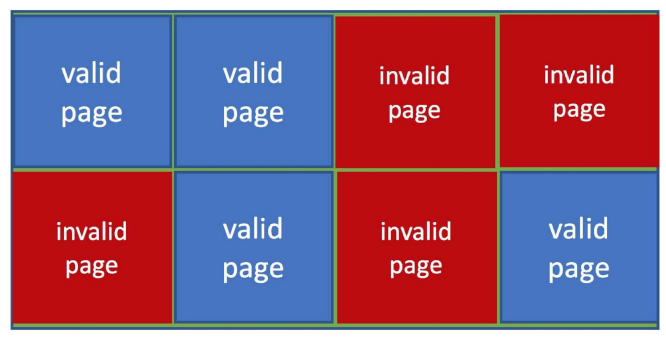
\includegraphics[width = .5\textwidth]{../res/imgs/mass memory/NAND_block.png}
    \caption{Un blocco con delle pagine valide e delle pagine non valide.}
    \label{fig:NAND_block}
\end{figure}
Alcuni dati infatti saranno aggiornati mentre degli altri dati sono più vecchi e non hanno più valore, di conseguenza sono dei candidati per essere rimpiazzati nel caso in cui fosse necessario dello spazio: è quindi presente un algoritmo di \textbf{garbage collection} che permette proprio di rimuovere delle pagine datate. Cosa succede però se tutti i blocchi hanno una o più pagine scritte? È necessario di un buffer dove il garbage collector sposta le pagine temporaneamente in modo da liberare lo spazio per poi ricopiare le pagine valide. Tipicamente una parte della NVM (circa il 20\%) è lasciata a disposizione del buffer per il garbage collector (\textit{overprovisioning}). Nel momento in cui arriva una nuova richiesta in scrittura e non c'è spazio, il garbage collector andrà a prendere le pagine e salvarle nel buffer, andrà a cancellare il blocco per poi ricopiare le pagine nuove nel blocco.

% 
\subsubsection{Memoria volatile}
Sono presenti casi, dove al fine di implementare dei file systems, sono necessario le memoria volatili, ovvero memoria che non mantiene salvati i dati quando manca l'alimentazione (ovvero quando il computer si spegne). Stiamo parlando dei \textbf{RAM drives}, che sono implementati attraverso memorie mantenute in vita solo quando l'alimentazione è disponibile. Tali memorie possono essere utilizzate per varie operazioni sfruttando il tempo di accesso molto rapido, come l'utilizzo di file temporanei.

% 
\subsubsection{Nastro magnetico}
Un'altra tecnologia meno comune nei computer di tutti i giorni ma che comunque rimane importante per altri dispositivi, come i server, è il cosiddetto  nastro magnetico. Questa è un'altra forma di memorizzazione su cui grandi moli di dati vengono immagazzinati, soprattutto per fare un \textbf{backup}. In questi nastri l'accesso ai dati è effettuato in modo \textbf{sequenziale}: se dobbiamo accedere ad una particolare zona del nastro è necessario scorrere tutto il nastro fino a che non si raggiunge la zona desiderata. È ovviamente molto inefficiente per un accesso di tipo random ma è efficiente per accessi sequenziali; proprio per questo motivo è ottimo per i backup. 

% 
\subsubsection{Dispositivi di memorizzazione esterna}
Discutiamo ora, brevemente, altre periferiche le quali possono essere collegate temporaneamente attraverso dei connettori (dei \textit{bus}) al computer. Le periferiche più famosi sono l'ATA, in particolare il SATA. Per invece per quanto riguarda i dispositivi NVM la loro velocità di trasferimento ha stimolato la creazione di connettori con standared più veloci 

% 
\subsection{Indirizzamento}
Nonostante le tecnologie sono implementate diversamente l'una dall'altra, dal punto di vista del computer i dispositivi sono molti simili, anche se i dispositivi fisici sono completamente diversi. Indipendentemente dal fatto che un file venga salvato su una SSD oppure su un HDD, questo verrà salvato sia su una periferica che sull'altra in quanto il computer non nota differenze tra un dispositivo e l'altro. È un concetto molto simile all'indirizzo logico e fisico per i processi, dove questi ultimi vedevano solo i loro indirizzi relativi senza sapere quale spazio in memoria sarebbe stato occupato. Analogamente il sistema operativo salva il file all'interno del dispositivo senza sapere come questo sia fatto. Sarà infatti compito del dispositivi tradurre i segnali dal sistema operativo in operazioni da effettuare nella specifica periferica.

Per esempio, la scrittura su un HDD potrebbe essere rappresentata logicamente come la scrittura su un array unico. Questo array è definito inserendo in maniera contigua tutti i cilindri di una traccia per poi proseguire con il cilindro della traccia più interna. IN questo modo tutti i dati presenti sui vari livelli del disco rigido sono rappresentati mediante un array. 

Avere una conoscenza di come il dispositivo funziona è comunque utile per il sistema operativo al fine di riuscire ad ottimizzare le operazioni da effettuare sulla periferica di archiviazione. Queste informazioni sono salvata nella \textbf{LBA}, ovvero il \textit{Logical Block Addres}.

% 
\subsection{HDD scheduling}
Tipicamente non c'è mai solo un processo che vuole accedere al disco ma ce ne sono di diversi. Di conseguenza il sistema operativo mantiene delle code che contengono i processi in attesa per l'accesso al disco. Nel momento in cui sono presenti delle code di attesa, sicuramente saranno presenti degli algoritmi che scelgono quale processo andrà ad effettuare l'accesso al disco. In questo caso si può sfruttare il fatto che spesso indirizzi LBA vicini corrispondono anche a indirizzi fisici vicini tra loro. 

% 
\subsubsection{FCFS}
Il primo algoritmo che andiamo a vedere è, di consueto, un algoritmo FIFO. Infatti, proprio come nel CPU scheduling (\ref{CPU scheduling}), FCFS sta per \textit{FIrst Come First Served}.
\begin{figure}[h]
    \centering
    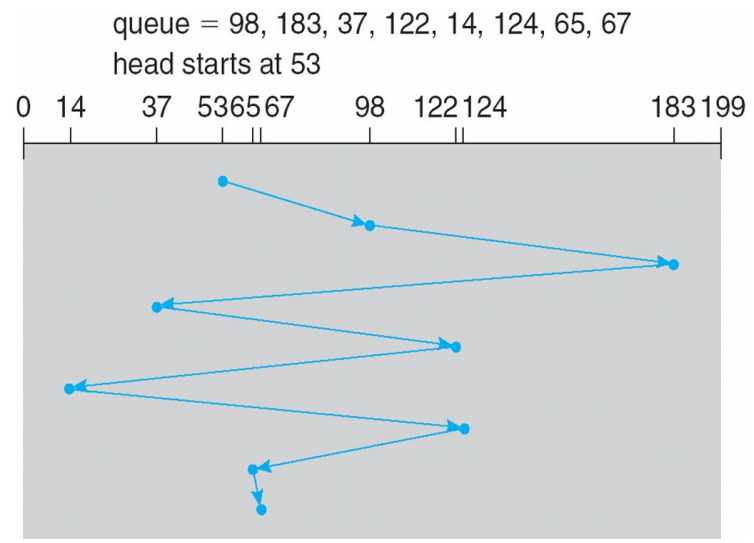
\includegraphics[width = .5\textwidth]{../res/imgs/mass memory/FCFS.png}
    \caption{Funzionamento dell'algoritmo FCFS.}
    \label{fig:FCFS_storage}
\end{figure}
 Con questo algoritmo si ha quindi una coda FIFO dove il primo processo che entra nella coda (e quindi fa la richiesta di accesso) sarà anche il primo ad uscire.Osserviamo la figura \ref{fig:FCFS_storage} e ipotizziamo che arrivi una serie di richieste che corrisponda ad andare nella traccia 98, poi nella traccia 183 e cosi' via fino alla traccia 67. Ipotizziamo di partire dalla traccia 53: andare a soddisfare le richieste in ordine FIFO significa spostare la testina lungo il disco e spostarsi da una traccia all'altra. Possiamo notare subito che questo algoritmo non tiene conto in alcun modo della prossimità delle tracce tra di loro, ma si basa solamente sull'ordine di entrata. Calcolando il numero di tracce che ha dovuto scorrere per completare la coda, scopriamo che il totale è di 640 tracce.

% 
\subsubsection{SSTF}
Un possibile miglioramento è il cosiddetto SSTF, che sta per \textit{Shortest Seek-Time First}: è un algoritmo simile al SJF del CPU scheduling (\ref{SJF}), dove si va a scegliere il processo che ha un burst time più basso. Analogamente in questo caso, si va a scegliere il processo meno distante rispetto alla posizione della testina, di conseguenza si va a soddisfare la richiesta che ci permette di saltare meno tracce. Osservando la figura \ref{fig:SSTF}, notiamo che l'ordine di esecuzione è diverso dal precedente in quanto dalla traccia 53 si passa alla 65, poi alla 67 e così via. In questo caso la distanza totale percorsa (in tracce) è di 236, che è un terzo rispetto a quella del FCFS.
\begin{figure}[h]
    \centering
    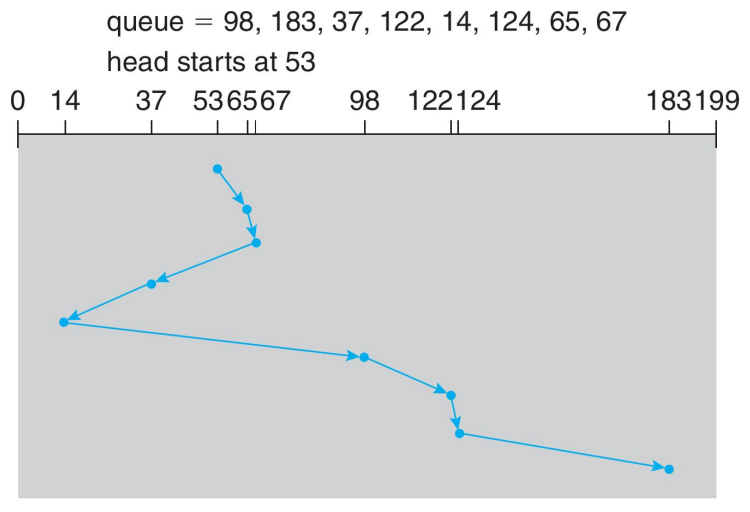
\includegraphics[width = .5\textwidth]{../res/imgs/mass memory/SSTF.png}
    \caption{Funzionamento dell'algoritmo SSTF.}
    \label{fig:SSTF}
\end{figure}
Proprio come nel caso dell'algoritmo SJF ci possono essere dei problemi di \textbf{starvation}, ovvero che arrivino sempre richieste vicine tra loro che vengono immediatamente soddisfatte trascurando una richiesta che è più lontana che potenzialmente non verrebbe mai eseguita. Ciò nonostante l'algoritmo rimane migliore rispetto al FCFS però, dato che si possono verificare questo tipo di situazioni, rimane un algoritmo non ottimale.

%
\subsubsection{SCAN e C-SCAN}\label{scan}
Al fine di evitare la starvation si è implementato l'algoritmo SCAN. Questo algoritmo è molto semplice: la testina va avanti e indietro lungo il disco e, mentre lo fa, soddisfa tutte le richieste che arrivano (figura \ref{fig:SCAN}). Il problema di questo algoritmo è che si ha uno soddisfacimento non equo delle richieste. Poniamo di trovarci nella traccia 10 e stiamo per arrivare alla 0 per poi tornare indietro. Se arriva una richiesta alla traccia 160 e dopo arrivano delle richieste alla traccia 31, 41, e 59, queste richieste verranno soddisfatte prima della richiesta alla traccia 160 la quale deve attendere più tempo anche se è arrivata prima delle altre.
\begin{figure}[h]
    \centering
    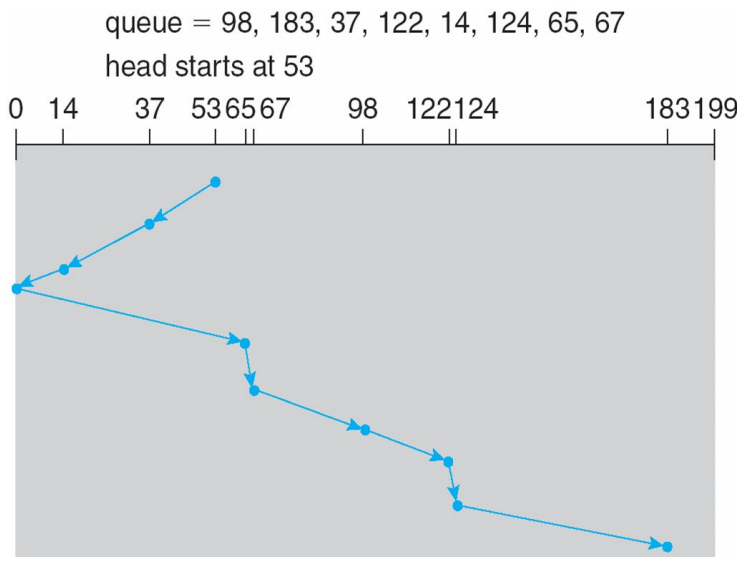
\includegraphics[width = .5\textwidth]{../res/imgs/mass memory/SCAN.png}
    \caption{Funzionamento dell'algoritmo SCAN.}
    \label{fig:SCAN}
\end{figure}

\noindent Per questo motivo si è implementato un altro algoritmo, molto simile, chiamato \textbf{Circular-SCAN} (C-SCAN). Questo algoritmo, al posto di andare avanti e indietro come l'algoritmo SCAN, una volta che arriva alla fine, alla traccia 199, non torna indietro soddisfacendo altre richieste ma va subito alla traccia 0 e ricomincia (figura \ref{fig:C-SCAN}). In questo caso però, anche se le richieste sono soddisfatte in maniere più equa, il tempo di ricerca totale è nettamente maggiore rispetto a quello dell'algoritmo SCAN.
\begin{figure}[h]
    \centering
    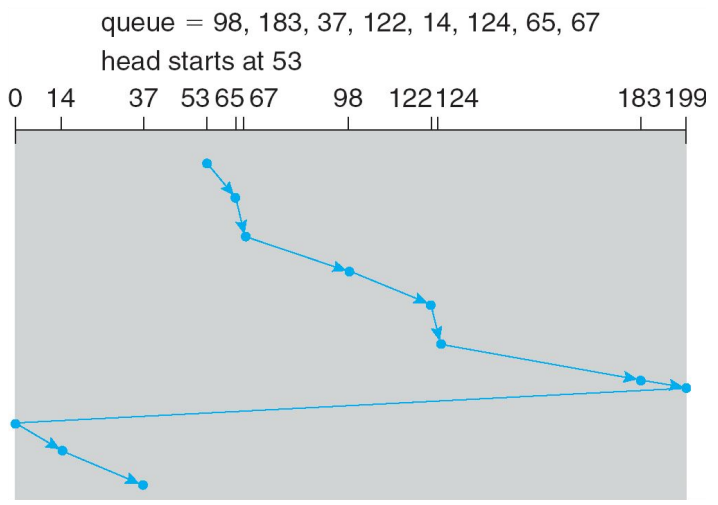
\includegraphics[width = .5\textwidth]{../res/imgs/mass memory/C-SCAN.png}
    \caption{Funzionamento dell'algoritmo C-SCAN.}
    \label{fig:C-SCAN}
\end{figure}

% 
\subsubsection{Scelta dell'algoritmo}
La scelta dell'algoritmo da utilizzare dipende sicuramente dal tipo di applicazione che si usano. Quelli discussi in questo capitolo sono gli algoritmi utilizzati più comunemente nei sistemi operativi. Generalmente SSTF è molto più utilizzato rispetto al FCFS mentre gli algoritmi SCAN e C-SCAN sono utilizzati nei sistemi con un alto carico di dati da memorizzare. 





